\documentclass[]{book}
\usepackage{indentfirst}
\usepackage[english]{babel}
\usepackage[utf8x]{inputenc}
\usepackage{pdfpages}
\usepackage{amsmath}
\usepackage{amssymb}
\usepackage{graphicx}
\usepackage{fancyhdr}
\usepackage[colorinlistoftodos]{todonotes}
\usepackage{float}
\usepackage{caption}
\usepackage{multicol}
\usepackage[notintoc]{nomencl}
\usepackage{lmodern}
\usepackage{subfiles}
\usepackage{setspace}
\usepackage[toc,page]{appendix}
\usepackage{apptools}
\usepackage{titlesec}
\usepackage{emptypage}
\usepackage{afterpage}
\pdfoptionpdfminorversion=7 %for pdfs
\usepackage{etoolbox}
\apptocmd{\sloppy}{\hbadness 10000\relax}{}{}
\emergencystretch=1em

%% CHAPTER TITLE FORMATTING
\titleformat{\chapter}[display]   
{\normalfont\huge\bfseries}{\chaptertitlename\ \thechapter}{20pt}{\huge}   
\titlespacing*{\chapter}{0pt}{-40pt}{20pt}
\titleformat{\chapter}[hang] 
{\normalfont\huge\bfseries}{\chaptertitlename\ \thechapter:}{1em}{} 

%APPENDIX FORMATTING
\AtAppendix{\titleformat{\chapter}[block]{\centering\huge\bfseries}{\appendixname~\thechapter:}{0.333em}{}%
	\titlespacing*{\chapter}{0pt}{-20pt}{20pt}}

\raggedbottom %wont scale to end of page

% WRAP CITATIONS
\usepackage{breakcites}
% MARGINS
\usepackage[margin=1in]{geometry}
% CHANGE THIS TO CHANGE THE TITLE
\newcommand{\reporttitle}{Capstone Report}
% THIS NEXT SECTION IS FOR CHANGING SECTION TITLE FONT SIZE
\usepackage{titlesec}
\titleformat{\section}
  {\normalfont\fontsize{16}{16}\bfseries}{\thesection}{1em}{}
\titleformat{\subsection}
  {\normalfont\fontsize{14}{14}\bfseries}{\thesubsection}{1em}{}
\titleformat{\subsubsection}
  {\normalfont\fontsize{12}{12}\bfseries}{\thesubsubsection}{1em}{}
\setcounter{secnumdepth}{4}
\setcounter{tocdepth}{4}
\titleformat{\paragraph}
{\normalfont\normalsize\bfseries}{\theparagraph}{1em}{}
\titlespacing*{\paragraph}
{0pt}{3.25ex plus 1ex minus .2ex}{1.5ex plus .2ex}
% SPACING 1.5
\linespread{1.5}
% SET TAB SIZE
\setlength\parindent{10mm}
% BIB
\usepackage[hyphens,spaces,obeyspaces]{url}
\usepackage[numbers]{natbib}
% SUMS
\makeatletter

\newcommand*\curveplus{%
  \mathbin{\rotatebox[origin=c]{90}{$\m@th\curvearrowleft$}+}}
\newcommand*\rightplus{%
  \mathpalette\@rightplus\relax}
\newcommand*\@rightplus[1]{%
  \mathbin{\vcenter{\hbox{$\m@th\overset{#1+}{\to}$}}}}

\newcommand*\upplus{%
  \mathbin{+\mathord\uparrow}}

\makeatother

%#####################################################################
%	BEGIN DOCUMENT
%#####################################################################

\begin{document}

%---------------------------------------------------------------------
%	BEGIN TITLE PAGE
%---------------------------------------------------------------------
\begin{titlepage}
\newcommand{\HRule}{\rule{\linewidth}{0.5mm}}
\center
 
%	HEADING SECTIONS
\textsc{\LARGE University of Ottawa}\\[1.5cm]
\textsc{\Large MCG4322}\\[0.5cm]
\textsc{\large RE3 - Wildcat Engineering}\\[0.5cm]

%	TITLE SECTION
\HRule \\[0.4cm]
{\huge \bfseries \reporttitle{}}\\
\HRule\\ [0.2cm]

\Large \textbf{Volume \textit{x} of \textit{y}} \\[1cm]

%	AUTHOR SECTION
\Large Joey Kane - 7386330\\
Isaak Goldenberg - 7395188\\
Sawyer Woodside - 7158568\\
Alex Pennell - 7334789\\[0.5cm]

%	DATE SECTION
{\large December 8, 2017}\\[0.5cm] % Change to Due Date of report

%	LOGO SECTION
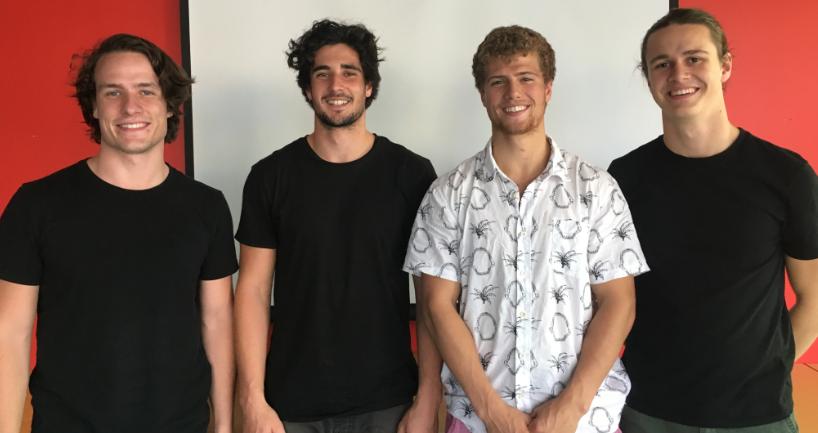
\includegraphics[width=0.8\textwidth]{img/general/boys.PNG}\\[0.5cm]

% 	SPONSOR SECTION
\large \emph{Sponsor:} Dr. Eric Lanteigne

\vfill
\end{titlepage}


\frontmatter

%---------------------------------------------------------------------
%	ABSTRACT
%---------------------------------------------------------------------
\chapter*{Abstract}
i.Contents of each book (if applicable) \\
ii.Description of design\\
iii.Special considerations\\
iv.Illustration of the final design
\\
half page, one paragraph
\pagebreak

%---------------------------------------------------------------------
%	TABLE OF CONTENTS
%---------------------------------------------------------------------
\tableofcontents

%---------------------------------------------------------------------
%	LIST OF FIGURES
%---------------------------------------------------------------------
\listoffigures
\pagebreak

%---------------------------------------------------------------------
%	LIST OF TABLES
%---------------------------------------------------------------------
\listoftables
\pagebreak

%#####################################################################
%	NOMENCLATURE
%#####################################################################
\cleardoublepage  
\renewcommand{\nomname}{Nomenclature}
\markboth{\MakeUppercase\nomname}{\MakeUppercase\nomname}  
\printnomenclature
  
  \nomenclature[]{$E_p$}{Modulus of elasticity of considered plastic hub or boss [$N/mm^2$]}
  \nomenclature[]{$\sigma_s$}{Allowable design stress for plastic, $N/mm^2$}
  \nomenclature[]{$\sigma_a$}{Hoop stress, [$N/mm^2$]}
  \nomenclature[]{$i_a$}{Allowable interference, [$mm$]}
  \nomenclature[]{$d_s$}{Shaft diameter, [$mm$]}
  \nomenclature[]{$d_s$}{Shaft diameter, [$mm$]}
  \nomenclature[]{$d_i$}{Interference diameter, [$mm$]}
  \nomenclature[]{$d_s$}{Hub outer diameter, [$mm$]}
  \nomenclature[]{$F_{spring}$}{Force applied by hinge spring, [$N$]}  
  \nomenclature[]{$T_w$}{Friction wheel motor torque, [$Nm$]}
  \nomenclature[]{$F_{nfric}$}{Normal force acting on friction wheel, [$N$]}  
  \nomenclature[]{$F_{ffric}$}{Friction force acting on friction wheel, [$N$]}
  \nomenclature[]{$F_g$}{Force of gravity, [$N$]}
  \nomenclature[]{$T_{spring}$}{Torque of hinge spring, [$Nm$]}
  \nomenclature[]{$L_s$}{Length from fastener to fastener of gondola motor to hinge, [$m$]} 
  \nomenclature[]{$L_{hs}$}{Distance from the pivot of the hinge to the gondola motor fastener, [$m$]}
  \nomenclature[]{$L_{hw}$}{Distance from the gondola motor fastener to the contact point of the friction wheel, [$m$]}
  \nomenclature[]{$\mu$}{Coefficient of friction}
  \nomenclature[]{$r_{fw}$}{Radius of friction wheel, [$m$]}  
  \nomenclature[]{$L_{rx}$}{Friction wheel motors shaft length, [$m$]}
  \nomenclature[]{$a_{airship}$}{Acceleration of airship, [$m/s$]}  
  \nomenclature[]{$m_{airship}$}{Mass of airship, [$kg$]}
  \nomenclature[]{$a_{gondola1}$}{Acceleration of Gondola 1 , [$m/s^2$]}
  \nomenclature[]{$a_{gondola2}$}{Acceleration of Gondola 2 , [$m/s^2$]}
  \nomenclature[]{$m_{gondola1}$}{Mass of Gondola 1, [$kg$]}
  \nomenclature[]{$m_{gondola2}$}{Mass of Gondola 2, [$kg$]}
  \nomenclature[]{$F_{s1}$}{Force on friction wheel motor fastener 1 , [$N$]}
  \nomenclature[]{$F_{s2}$}{Force on friction wheel motor fastener 2 , [$N$]}
  \nomenclature[]{$F_{a}$}{Force on fastener a (hinge to gondola), [$N$]}
  \nomenclature[]{$F_{b}$}{Force on fastener b (hinge to gondola), [$N$]}
  \nomenclature[]{$F_{\alpha}$}{Force on fastener $\alpha$ (hinge to gondola), [$N$]}
  \nomenclature[]{$F_{\beta}$}{Force on fastener $\beta$ (hinge to gondola), [$N$]}
  \nomenclature[]{$L_a$}{Length from pivot point of hinge to fastener a , [$m$]}
  \nomenclature[]{$L_b$}{Length from pivot point of hinge to fastener b , [$m$]}
  \nomenclature[]{$L_{contact}$}{Length from contact to contact of bearings on keel, [$m$]}
  \nomenclature[]{$F_{NB}$}{Normal force applied to bearing, [$N$]}
  \nomenclature[]{$L_G$}{Width of gondola, [$m$]}
  \nomenclature[]{$L_{bc}$}{Length from centerline of gondola to fastener b, [$m$]}
  \nomenclature[]{$L_{ac}$}{Length from centerline of gondola to fastener a, [$m$]}
  \nomenclature[]{$R$}{Reaction force, [$N$]}
  \nomenclature[]{$L_{drive}$}{Length of gondola hinge to friction wheel contact, [$m$]}
  \nomenclature[]{$L_{cm}$}{Length from gondola wall to center of mass of gondola, [$m$]}
  \nomenclature[]{$L_m$}{Length from side of gondola to gondola drive motor hinge, [$m$]}
  \nomenclature[]{$H_{keel}$}{Height of the bearing arm contact point on the keel, [$m$]}
  \nomenclature[]{$F_{LA}$}{Linear actuator force, [$N$]}
  \nomenclature[]{$F_{brake}$}{Normal braking force keel reaction, [$N$]}
  \nomenclature[]{$W_{LA}$}{Weight of linear actuator, [$N$]}
  \nomenclature[]{$F_{GR}$}{Reaction force of gondola, [$N$]}
  \nomenclature[]{$F_T$}{Thruster force, [$N$]}
  \nomenclature[]{$W_T$}{Weight of thruster, [$N$]}
  \nomenclature[]{$W_A$}{Weight of thruster assembly arm, [$N$]}
  \nomenclature[]{$W_E$}{Weight of thruster enclosure, [$N$]}
  \nomenclature[]{$F_R$}{Keel to assembly arm connector reaction, [$N$]}
  \nomenclature[]{$M_R$}{Connector moment reaction, [$Nm$]}
  \nomenclature[]{$W_c$}{Weight of connection piece, [$N$]}
  \nomenclature[]{$F_{K1}$}{Keel reaction force 1, [$N$]}
  \nomenclature[]{$F_{K2}$}{Keel reaction force 2, [$N$]}
  \nomenclature[]{$F_{c1}$}{Connector moment couple force 1, [$N$]}
  \nomenclature[]{$F_{c2}$}{Connector moment couple force 2, [$N$]}
  \nomenclature[]{$c$}{Distance from neutral axis to stress location, [$m$]}
  \nomenclature[]{$w_{army}$}{Width of the bearing arm in the y direction, [$m$]}
  \nomenclature[]{$w_{armx}$}{Width of the bearing arm in the x direction, [$m$]}
  \nomenclature[]{$F_{bolt}$}{Bolt pretension force, [$N$]}
  \nomenclature[]{$\sigma _{washer}$}{Compressive force of washer, [$Pa$]}
  \nomenclature[]{$\sigma _{x}$}{Principle stress, [$Pa$]}  
  \nomenclature[]{$\sigma '$}{Von Mises Stress, [$Pa$]}
  \nomenclature[]{$S_{compressive}$}{Compressive strength of gondola material, [$Pa$]}
  \nomenclature[]{$\eta$}{Safety Factor}
  \nomenclature[]{$L_{SF}$}{Length to snap fit bearing, [$m$]}
  \nomenclature[]{$M_1$}{Reaction moment on bearing arm, [$Nm$]}
  \nomenclature[]{$F_{RSF}$}{Force of snap fit bearing [$N$]}
    
%---------------------------------------------------------------------
%	MAIN BODY
%---------------------------------------------------------------------
\pagestyle{fancy}
\setlength{\headheight}{14.5pt} 
\fancyhf{}
\rhead{\rightmark}
\cfoot{\thepage}

\mainmatter

%#####################################################################
%	INTRODUCTION
%#####################################################################
\subfile{./tex/chapter1Introduction.tex}

%#####################################################################
%	PROPOSED DESIGN
%#####################################################################
\subfile{./tex/chapter2ProposedDesign.tex}

%#####################################################################
%	ANALYSIS
%#####################################################################
\subfile{./tex/chapter3Analysis.tex}

%#####################################################################
%	BIBLIOGRAPHY
%#####################################################################
\bibliographystyle{plainnat}
\bibliography{library}

\pagebreak

%#####################################################################
%	APPENDIX
%#####################################################################
\subfile{./tex/appendix.tex}

\end{document}